\documentclass{beamer}

\input{settings.tex}


\title{Linear inequalities and polytopes}
\subtitle{Computational Intelligence, Lecture 5}
\author{by Sergei Savin}
\centering
\date{\mydate}

\begin{document}
\maketitle


\begin{frame}{Content}

\begin{itemize}
\item Convex polytopes
\item Half-spaces
\item H-representation
\item V-representation
\item G-representation (Zonotopes)
\item Linear approximation of convex regions
\end{itemize}

\end{frame}



\begin{frame}{Convex polytopes}
% \framesubtitle{Parameter estimation}
\begin{flushleft}

Before defining what a convex polytope is, let us look at examples:

\include{fig1}
 
\end{flushleft}
\end{frame}


\begin{frame}{Convex polytopes}
% \framesubtitle{Parameter estimation}
\begin{flushleft}

You can think of polytopes as geometric figures (or continuous sets of points) with linear edges, faces and higher-dimensional analogues.

\bigskip

\begin{definition}
 Convex polytopes are polytopes whose every two points can be connected with a line that would lie in the polytope. They can be bounded or unbounded.
\end{definition}
 
\end{flushleft}
\end{frame}


\begin{frame}{Half-spaces}
\framesubtitle{Definition}
\begin{flushleft}

We can define half-space as a set of all points $\mathbf{x}$, such that $\mathbf{a}^\top \mathbf{x} \leq b$. It has a very clear geometric interpretation. In the following image, the filled space is \textbf{not} in the half space.

\include{fig2}
 
\end{flushleft}
\end{frame}



\begin{frame}{Half-spaces}
\framesubtitle{Construction. Simple case}
\begin{flushleft}

Consider half-space that passes through the origin, and defined by its normal vector $\mathbf{n}$:

\include{fig3}

It is easy to see that this half-space can be defined as "all vectors $\mathbf{x}$, such that $\mathbf{n} \cdot \mathbf{x} \leq 0$", which is the same as using $\mathbf{n}$ instead of $\mathbf{a}$ in our original definition, setting $b = 0$.
 
\end{flushleft}
\end{frame}




\begin{frame}{Half-spaces}
\framesubtitle{Construction. General case}
\begin{flushleft}

In the general case there is some distance between the boundary of the half-space and the origin, let's say $d$.

\include{fig4}
%
Here the half space can be defined as "all vectors $\mathbf{x}$, such that $\mathbf{x}^\top \frac{\mathbf{n}}{|| \mathbf{n} ||}  \leq d$". This is the same as making $\mathbf{a} = \mathbf{n}$ and $b = d ||\mathbf{a}||$.
 
\end{flushleft}
\end{frame}



\begin{frame}{Half-spaces}
\framesubtitle{Combination}
\begin{flushleft}

We can define a region of space as an \emph{intersection} of half-spaces $\mathbf{a}_i^\top \mathbf{x} \leq b_i$:

\include{fig5}

Resulting region will be easily described as $\begin{bmatrix} \mathbf{a}_1^\top \\ ... \\ \mathbf{a}_k^\top \end{bmatrix} \mathbf{x} \leq \begin{bmatrix} b_1 \\ ... \\ b_k \end{bmatrix}$

 
\end{flushleft}
\end{frame}


\begin{frame}{H-representation of a polytope}
%\framesubtitle{}
\begin{flushleft}

The last result allows us to write any convex polytope as a matrix inequality:

\begin{equation}
\label{eq:ineq} 
    \mathbf{A} \mathbf{x} \leq  \mathbf{b} 
\end{equation}

And conversely, any matrix inequality \eqref{eq:ineq} represents either an empty set or a convex polytope.

\bigskip

\begin{definition}
 $\mathbf{A} \mathbf{x} \leq  \mathbf{b}$ is called \emph{H-representation} (half-space representation) of a polytope.
\end{definition}
 
\end{flushleft}
\end{frame}



\begin{frame}{H-representation in COP}
	%\framesubtitle{}
	\begin{flushleft}
		
		We can use containment in an H-polytope as a part of convex optimation problem. For example, the following QP includes such constraint:
		
		\begin{equation}
			\begin{aligned}
				& \underset{\mathbf{x}}{\text{minimize}}
				& & \mathbf{x}^\top \mathbf{H} \mathbf{x} + \mathbf{f}^\top\mathbf{x}, \\
				& \text{subject to}
				& & \mathbf{A}\mathbf{x} \leq \mathbf{b}.
			\end{aligned}
		\end{equation}
		
	\end{flushleft}
\end{frame}









\begin{frame}{V-representation}
% \framesubtitle{}
\begin{flushleft}

Convex polytopes have alternative representations, such as \emph{V-representation}. It amounts to representing polytope as a set of its vertices.

\begin{example}
$V = \begin{bmatrix} -1 & -1 & 1 & 1 \\ -1 & 1 & 1 & -1 \end{bmatrix}$ is a V-representation of a square.
\end{example}

\begin{example}
$\begin{bmatrix} 1 & 0 \\ 0 & 1 \\ -1 & 0 \\ 0 & -1 \end{bmatrix}
\begin{bmatrix} x_1 \\ x_2 \end{bmatrix} \leq
\begin{bmatrix} 1 \\ 1 \\ 1 \\ 1 \end{bmatrix}$
is an H-representation of the same square.
\end{example}
 
\end{flushleft}
\end{frame}


\begin{frame}{Convex hull}
	% \framesubtitle{Parameter estimation}
	\begin{flushleft}
		
		Given points $\bo{x}_1$, $\bo{x}_2$, ..., $\bo{x}_N$ their convex hull is represented as:
		
		\begin{equation}
			\mathcal{P} = \left \{  \bo{x} = \sum_{i=1}^{N} \alpha_i\bo{x}_i: \   \sum_{i=1}^{N} \alpha_i = 1, \  \alpha_i  \in [0 \ 1] \right \}
		\end{equation}
		
		See Appendix for an illustration of this formula.
		
	\end{flushleft}
\end{frame}



\begin{frame}{V-representation in COP}
	%\framesubtitle{}
	\begin{flushleft}
		
		We can use containment in an V-polytope as a part of convex optimation problem. For example, the following QP includes such constraint:
		
		\begin{equation}
			\begin{aligned}
				& \underset{\mathbf{x}}{\text{minimize}}
				& & \mathbf{x}^\top \mathbf{H} \mathbf{x} + \mathbf{f}^\top\mathbf{x}, \\
				& \text{subject to}
				& & \begin{cases}
					\mathbf{x} = \sum\limits_{i=1}^{n} \alpha_i  \mathbf{v}_i, \\
					\sum\limits_{i=1}^{n} \alpha_i = 1, \\
					\alpha_i \geq 0.
				\end{cases}
			\end{aligned}
		\end{equation}
		
		Notice that the constraint amounts to equating $\mathbf{x}$ to a convex combination of the vertices of the V-polytope.
		
	\end{flushleft}
\end{frame}



\begin{frame}{H and V-representations}
% \framesubtitle{}
\begin{flushleft}

To transfer from H-representation to V-representation, you need to solve \emph{vertex enumeration} problem, which is computationally expensive. 

\bigskip

It is also possible to construct H-representation out of V-representation.  Both algorithms are not convex.
 
\end{flushleft}
\end{frame}




\begin{frame}{Zonotopes: G-representation}
	% \framesubtitle{}
	\begin{flushleft}
		
		A zonotope $\mathcal{Z}$ is a symmetric polytope defined by its \emph{center} $\bo{c}$ and \emph{generator} $\bo{G}$:
		
		\begin{equation}
			\mathcal{Z} = \{ \bo{x}: \ \bo{x}=\bo{G}\beta+\bo{c}, \ ||\beta||_\infty \leq 1  \}
		\end{equation}
	
		The set $\{ \beta: \ ||\beta||_\infty \leq 1  \}$ is a hypercube and zonotope $\mathcal{Z}$ is a projection (shadow) of this hypercube onto a lower-dimensional space; the projection is defined by the matrix $\bo{G}$.
		
		% TODO: \usepackage{graphicx} required
		\begin{figure}
			\centering
			\includegraphics[width=0.4\linewidth]{zonotope_example}
			\caption{Zonotope (\bref{https://www.researchgate.net/publication/322671928_Methods_for_order_reduction_of_zonotopes}{Source}) }
			\label{fig:zonotopeexample}
		\end{figure}
		%https://www.researchgate.net/publication/322671928_Methods_for_order_reduction_of_zonotopes
		
		
	\end{flushleft}
\end{frame}




\begin{frame}{G-representation in COP}
	%\framesubtitle{}
	\begin{flushleft}
		
		We can use containment in an G-polytope as a part of convex optimation problem. For example, the following QP includes such constraint:
		
		\begin{equation}
			\begin{aligned}
				& \underset{\mathbf{x}}{\text{minimize}}
				& & \mathbf{x}^\top \mathbf{H} \mathbf{x} + \mathbf{f}^\top\mathbf{x}, \\
				& \text{subject to}
				& & \begin{cases}
					\mathbf{x} = \bo{G}\beta+\bo{c}, \\
					-1 \geq \beta_i \geq 1.
				\end{cases}
			\end{aligned}
		\end{equation}
		
	\end{flushleft}
\end{frame}




\begin{frame}{Linear approximation of convex regions}
% \framesubtitle{Parameter estimation}
\begin{flushleft}
Some convex regions can be easily approximated using polytopes.

\include{fig6}

Which allows to represent constraints on $\mathbf{x}$ to belong in such a region as a matrix inequality
 
\end{flushleft}
\end{frame}



\begin{frame}{Exercise}
% \framesubtitle{Parameter estimation}
\begin{flushleft}

Write H-representation of the following polytopes:

\begin{itemize}
    \item Equilateral triangle
    \item Square
    \item Parallelepiped
    \item Trapezoid
\end{itemize}

\end{flushleft}
\end{frame}


% \begin{frame}{Self-study}
% % \framesubtitle{Part 3}
% \begin{flushleft}

% \begin{itemize}
%     \item \href{https://www.youtube.com/watch?v=kcOodzDGV4c}{Convex Optimization, lecture 3, S. Boyd. Stanford. Convex functions}.
% \end{itemize}

% \end{flushleft}
% \end{frame}

\myqrframe





\begin{frame}{Appendix A - convex hull, 1}
	% \framesubtitle{Parameter estimation}
	\begin{flushleft}
		
		
		\begin{figure}[.45\textwidth]
			\centering
			\resizebox{.65\textwidth}{!}
			{


\tikzset{every picture/.style={line width=0.75pt}} %set default line width to 0.75pt        

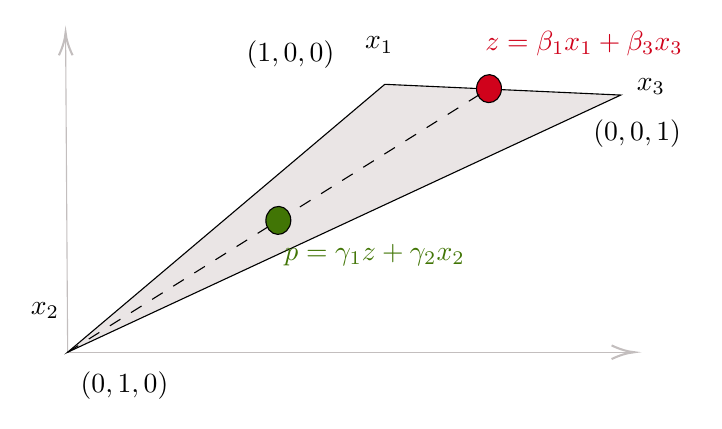
\begin{tikzpicture}[x=0.75pt,y=0.75pt,yscale=-1,xscale=1]
	%uncomment if require: \path (0,300); %set diagram left start at 0, and has height of 300
	
	%Straight Lines [id:da574149972137515] 
	\draw [color={rgb, 255:red, 195; green, 190; blue, 190 }  ,draw opacity=1 ]   (33,258.5) -- (304,258.5) ;
	\draw [shift={(306,258.5)}, rotate = 180] [color={rgb, 255:red, 195; green, 190; blue, 190 }  ,draw opacity=1 ][line width=0.75]    (10.93,-3.29) .. controls (6.95,-1.4) and (3.31,-0.3) .. (0,0) .. controls (3.31,0.3) and (6.95,1.4) .. (10.93,3.29)   ;
	%Straight Lines [id:da6051947502547008] 
	\draw [color={rgb, 255:red, 195; green, 190; blue, 190 }  ,draw opacity=1 ]   (33,258.5) -- (32.01,106.5) ;
	\draw [shift={(32,104.5)}, rotate = 89.63] [color={rgb, 255:red, 195; green, 190; blue, 190 }  ,draw opacity=1 ][line width=0.75]    (10.93,-3.29) .. controls (6.95,-1.4) and (3.31,-0.3) .. (0,0) .. controls (3.31,0.3) and (6.95,1.4) .. (10.93,3.29)   ;
	%Shape: Right Triangle [id:dp9642640346709239] 
	\draw  [fill={rgb, 255:red, 234; green, 229; blue, 229 }  ,fill opacity=1 ] (299.48,134.6) -- (33,258.5) -- (185.8,129.42) -- cycle ;
	%Shape: Ellipse [id:dp24503782326315404] 
	\draw  [fill={rgb, 255:red, 208; green, 2; blue, 27 }  ,fill opacity=1 ] (230.01,131.2) .. controls (230.19,127.48) and (233.02,124.6) .. (236.33,124.76) .. controls (239.64,124.92) and (242.18,128.07) .. (241.99,131.8) .. controls (241.81,135.52) and (238.98,138.4) .. (235.67,138.24) .. controls (232.36,138.08) and (229.82,134.93) .. (230.01,131.2) -- cycle ;
	%Straight Lines [id:da21833955225597546] 
	\draw  [dash pattern={on 4.5pt off 4.5pt}]  (33,258.5) -- (236,131.5) ;
	%Shape: Ellipse [id:dp28236760411930684] 
	\draw  [fill={rgb, 255:red, 65; green, 117; blue, 5 }  ,fill opacity=1 ] (128.51,194.7) .. controls (128.69,190.98) and (131.52,188.1) .. (134.83,188.26) .. controls (138.14,188.42) and (140.68,191.57) .. (140.49,195.3) .. controls (140.31,199.02) and (137.48,201.9) .. (134.17,201.74) .. controls (130.86,201.58) and (128.32,198.43) .. (128.51,194.7) -- cycle ;
	
	% Text Node
	\draw (118,107.4) node [anchor=north west][inner sep=0.75pt]    {$( 1,0,0)$};
	% Text Node
	\draw (285,145.4) node [anchor=north west][inner sep=0.75pt]    {$( 0,0,1)$};
	% Text Node
	\draw (38,266.4) node [anchor=north west][inner sep=0.75pt]    {$( 0,1,0)$};
	% Text Node
	\draw (175,105.4) node [anchor=north west][inner sep=0.75pt]    {$x_{1}$};
	% Text Node
	\draw (306,125.4) node [anchor=north west][inner sep=0.75pt]    {$x_{3}$};
	% Text Node
	\draw (14,233.4) node [anchor=north west][inner sep=0.75pt]    {$x_{2}$};
	% Text Node
	\draw (233,102.4) node [anchor=north west][inner sep=0.75pt]  [color={rgb, 255:red, 208; green, 2; blue, 27 }  ,opacity=1 ]  {$z=\beta _{1} x_{1} +\beta _{3} x_{3} \ $};
	% Text Node
	\draw (136.17,205.14) node [anchor=north west][inner sep=0.75pt]  [color={rgb, 255:red, 65; green, 117; blue, 5 }  ,opacity=1 ]  {$p=\gamma _{1} z+\gamma _{2} x_{2}$};
	
	
\end{tikzpicture}
}
		\end{figure}
		
		Let us illustrate the convex combination formula. 
		Let $\mathcal{P}$ be convex hull of points $\bo{x}_1$, $\bo{x}_2$ and $\bo{x}_3$:
		
		
		\begin{equation}
			\mathcal{P} = \left \{  \bo{x} = \sum_{i=1}^{3} \alpha_i\bo{x}_i: \   \sum_{i=1}^{3} \alpha_i = 1, \  \alpha_i  \in [0 \ 1] \right \}
		\end{equation}
		
		Let $\bo{z}$ be a convex combination of $\bo{x}_1$ and $\bo{x}_3$: $\bo{z} = \beta_1 \bo{x}_1 + \beta_3 \bo{x}_3 $. Then any $\bo{p} \in \mathcal{P}$ is expressed as a convex combination of $\bo{z}$ and $\bo{x}_2$: $\bo{p} = \gamma_1 \bo{z} + \gamma_2 \bo{x}_2$.
		
	\end{flushleft}
\end{frame}



\begin{frame}{Appendix A - convex hull, 2}
	% \framesubtitle{Parameter estimation}
	\begin{flushleft}
		
		
		
		\begin{figure}[.45\textwidth]
			\centering
			\resizebox{.45\textwidth}{!}
			{


\tikzset{every picture/.style={line width=0.75pt}} %set default line width to 0.75pt        

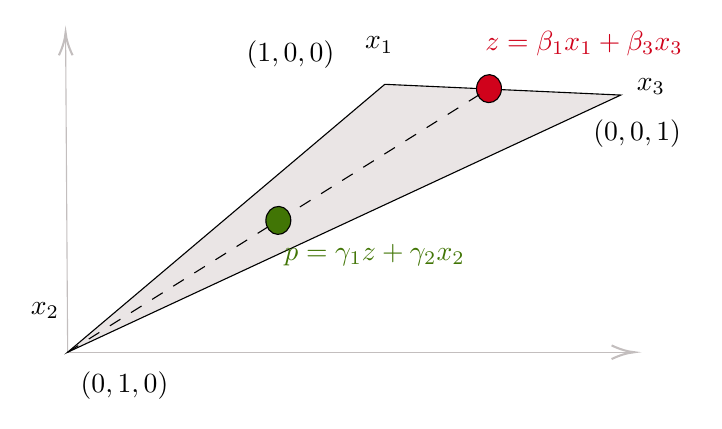
\begin{tikzpicture}[x=0.75pt,y=0.75pt,yscale=-1,xscale=1]
	%uncomment if require: \path (0,300); %set diagram left start at 0, and has height of 300
	
	%Straight Lines [id:da574149972137515] 
	\draw [color={rgb, 255:red, 195; green, 190; blue, 190 }  ,draw opacity=1 ]   (33,258.5) -- (304,258.5) ;
	\draw [shift={(306,258.5)}, rotate = 180] [color={rgb, 255:red, 195; green, 190; blue, 190 }  ,draw opacity=1 ][line width=0.75]    (10.93,-3.29) .. controls (6.95,-1.4) and (3.31,-0.3) .. (0,0) .. controls (3.31,0.3) and (6.95,1.4) .. (10.93,3.29)   ;
	%Straight Lines [id:da6051947502547008] 
	\draw [color={rgb, 255:red, 195; green, 190; blue, 190 }  ,draw opacity=1 ]   (33,258.5) -- (32.01,106.5) ;
	\draw [shift={(32,104.5)}, rotate = 89.63] [color={rgb, 255:red, 195; green, 190; blue, 190 }  ,draw opacity=1 ][line width=0.75]    (10.93,-3.29) .. controls (6.95,-1.4) and (3.31,-0.3) .. (0,0) .. controls (3.31,0.3) and (6.95,1.4) .. (10.93,3.29)   ;
	%Shape: Right Triangle [id:dp9642640346709239] 
	\draw  [fill={rgb, 255:red, 234; green, 229; blue, 229 }  ,fill opacity=1 ] (299.48,134.6) -- (33,258.5) -- (185.8,129.42) -- cycle ;
	%Shape: Ellipse [id:dp24503782326315404] 
	\draw  [fill={rgb, 255:red, 208; green, 2; blue, 27 }  ,fill opacity=1 ] (230.01,131.2) .. controls (230.19,127.48) and (233.02,124.6) .. (236.33,124.76) .. controls (239.64,124.92) and (242.18,128.07) .. (241.99,131.8) .. controls (241.81,135.52) and (238.98,138.4) .. (235.67,138.24) .. controls (232.36,138.08) and (229.82,134.93) .. (230.01,131.2) -- cycle ;
	%Straight Lines [id:da21833955225597546] 
	\draw  [dash pattern={on 4.5pt off 4.5pt}]  (33,258.5) -- (236,131.5) ;
	%Shape: Ellipse [id:dp28236760411930684] 
	\draw  [fill={rgb, 255:red, 65; green, 117; blue, 5 }  ,fill opacity=1 ] (128.51,194.7) .. controls (128.69,190.98) and (131.52,188.1) .. (134.83,188.26) .. controls (138.14,188.42) and (140.68,191.57) .. (140.49,195.3) .. controls (140.31,199.02) and (137.48,201.9) .. (134.17,201.74) .. controls (130.86,201.58) and (128.32,198.43) .. (128.51,194.7) -- cycle ;
	
	% Text Node
	\draw (118,107.4) node [anchor=north west][inner sep=0.75pt]    {$( 1,0,0)$};
	% Text Node
	\draw (285,145.4) node [anchor=north west][inner sep=0.75pt]    {$( 0,0,1)$};
	% Text Node
	\draw (38,266.4) node [anchor=north west][inner sep=0.75pt]    {$( 0,1,0)$};
	% Text Node
	\draw (175,105.4) node [anchor=north west][inner sep=0.75pt]    {$x_{1}$};
	% Text Node
	\draw (306,125.4) node [anchor=north west][inner sep=0.75pt]    {$x_{3}$};
	% Text Node
	\draw (14,233.4) node [anchor=north west][inner sep=0.75pt]    {$x_{2}$};
	% Text Node
	\draw (233,102.4) node [anchor=north west][inner sep=0.75pt]  [color={rgb, 255:red, 208; green, 2; blue, 27 }  ,opacity=1 ]  {$z=\beta _{1} x_{1} +\beta _{3} x_{3} \ $};
	% Text Node
	\draw (136.17,205.14) node [anchor=north west][inner sep=0.75pt]  [color={rgb, 255:red, 65; green, 117; blue, 5 }  ,opacity=1 ]  {$p=\gamma _{1} z+\gamma _{2} x_{2}$};
	
	
\end{tikzpicture}
}
		\end{figure}
		
		We can express $\bo{p}$ as:
		%
		\begin{align}
			\bo{p} =  \gamma_1 \bo{z} + \gamma_2 \bo{x}_2 
			           = \gamma_1 (\beta_1 \bo{x}_1 + \beta_3 \bo{x}_3 )+ \gamma_2 \bo{x}_2
		\end{align}
		%
		We can define $\alpha_1 = \gamma_1 \beta_1$, $\alpha_2= \gamma_2 \bo{x}_2$ and $\alpha_3 = \gamma_1 \beta_3$. Since $\gamma_i \geq 0$ and $\beta_i \geq 0$, we conclude that $\alpha_i \geq 0$.
		
		\bigskip
		
		We can show that $e = \alpha_1 + \alpha_2+\alpha_3 = 1$:
		%
		\begin{align}
			e =  \gamma_1(\beta_1 +\beta_3) + \gamma_2 = \gamma_1 + \gamma_2 = 1
		\end{align}
		
		
	\end{flushleft}
\end{frame}




\begin{frame}{Appendix A - convex hull, 3}
	% \framesubtitle{Parameter estimation}
	\begin{flushleft}
		
		
					\begin{figure}
							\begin{subfigure}{.5\textwidth}
									\centering
									\resizebox{.95\textwidth}{!}
									{


\tikzset{every picture/.style={line width=0.75pt}} %set default line width to 0.75pt        

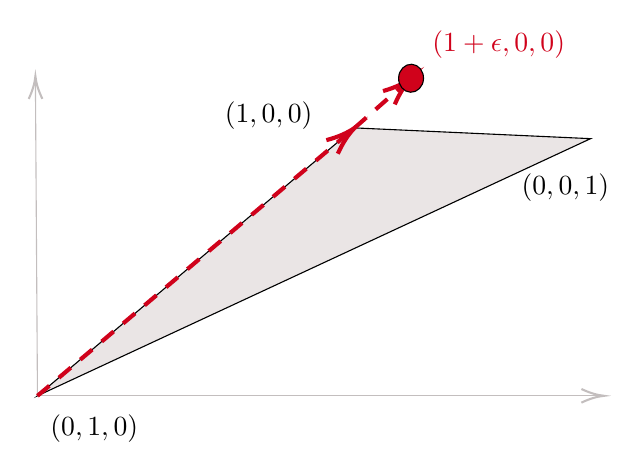
\begin{tikzpicture}[x=0.75pt,y=0.75pt,yscale=-1,xscale=1]
	%uncomment if require: \path (0,300); %set diagram left start at 0, and has height of 300
	
	%Straight Lines [id:da19398531606138758] 
	\draw [color={rgb, 255:red, 195; green, 190; blue, 190 }  ,draw opacity=1 ]   (33,258.5) -- (304,258.5) ;
	\draw [shift={(306,258.5)}, rotate = 180] [color={rgb, 255:red, 195; green, 190; blue, 190 }  ,draw opacity=1 ][line width=0.75]    (10.93,-3.29) .. controls (6.95,-1.4) and (3.31,-0.3) .. (0,0) .. controls (3.31,0.3) and (6.95,1.4) .. (10.93,3.29)   ;
	%Straight Lines [id:da8915945917872681] 
	\draw [color={rgb, 255:red, 195; green, 190; blue, 190 }  ,draw opacity=1 ]   (33,258.5) -- (32.01,106.5) ;
	\draw [shift={(32,104.5)}, rotate = 89.63] [color={rgb, 255:red, 195; green, 190; blue, 190 }  ,draw opacity=1 ][line width=0.75]    (10.93,-3.29) .. controls (6.95,-1.4) and (3.31,-0.3) .. (0,0) .. controls (3.31,0.3) and (6.95,1.4) .. (10.93,3.29)   ;
	%Shape: Right Triangle [id:dp8483033950517145] 
	\draw  [fill={rgb, 255:red, 234; green, 229; blue, 229 }  ,fill opacity=1 ] (299.48,134.6) -- (33,258.5) -- (185.8,129.42) -- cycle ;
	%Straight Lines [id:da6127334324636506] 
	\draw [color={rgb, 255:red, 208; green, 2; blue, 27 }  ,draw opacity=1 ][line width=1.5]  [dash pattern={on 5.63pt off 4.5pt}]  (33,258.5) -- (183.51,131.35) ;
	\draw [shift={(185.8,129.42)}, rotate = 139.81] [color={rgb, 255:red, 208; green, 2; blue, 27 }  ,draw opacity=1 ][line width=1.5]    (14.21,-4.28) .. controls (9.04,-1.82) and (4.3,-0.39) .. (0,0) .. controls (4.3,0.39) and (9.04,1.82) .. (14.21,4.28)   ;
	%Straight Lines [id:da19864673694857093] 
	\draw [color={rgb, 255:red, 208; green, 2; blue, 27 }  ,draw opacity=1 ][line width=1.5]  [dash pattern={on 5.63pt off 4.5pt}]  (185.8,129.42) -- (210.75,107.48) ;
	\draw [shift={(213,105.5)}, rotate = 138.67] [color={rgb, 255:red, 208; green, 2; blue, 27 }  ,draw opacity=1 ][line width=1.5]    (14.21,-4.28) .. controls (9.04,-1.82) and (4.3,-0.39) .. (0,0) .. controls (4.3,0.39) and (9.04,1.82) .. (14.21,4.28)   ;
	%Shape: Ellipse [id:dp19860722292637645] 
	\draw  [fill={rgb, 255:red, 208; green, 2; blue, 27 }  ,fill opacity=1 ] (207.01,105.2) .. controls (207.19,101.48) and (210.02,98.6) .. (213.33,98.76) .. controls (216.64,98.92) and (219.18,102.07) .. (218.99,105.8) .. controls (218.81,109.52) and (215.98,112.4) .. (212.67,112.24) .. controls (209.36,112.08) and (206.82,108.93) .. (207.01,105.2) -- cycle ;
	
	% Text Node
	\draw (222,81.4) node [anchor=north west][inner sep=0.75pt]  [color={rgb, 255:red, 208; green, 2; blue, 27 }  ,opacity=1 ]  {$( 1+\epsilon ,0,0)$};
	% Text Node
	\draw (122,115.4) node [anchor=north west][inner sep=0.75pt]    {$( 1,0,0)$};
	% Text Node
	\draw (265,150.4) node [anchor=north west][inner sep=0.75pt]    {$( 0,0,1)$};
	% Text Node
	\draw (38,266.4) node [anchor=north west][inner sep=0.75pt]    {$( 0,1,0)$};
	
	
\end{tikzpicture}
}
%									\label{fig:sfig1}
								\end{subfigure}%
							\begin{subfigure}{.5\textwidth}
									\centering
									\resizebox{.95\textwidth}{!}
									{


\tikzset{every picture/.style={line width=0.75pt}} %set default line width to 0.75pt        

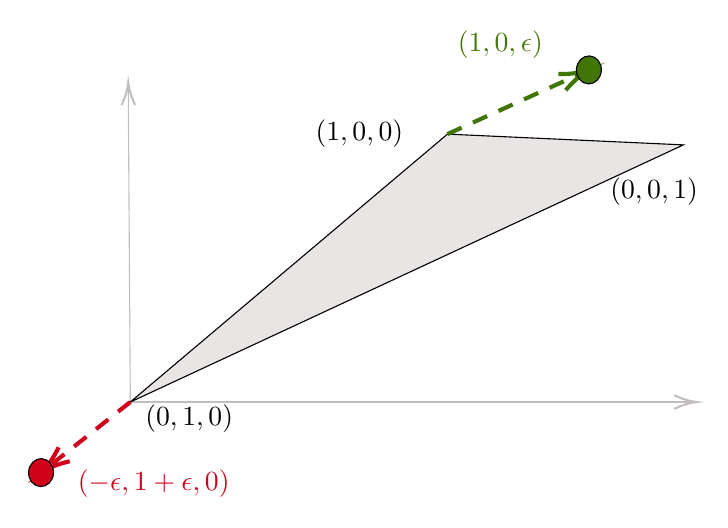
\begin{tikzpicture}[x=0.75pt,y=0.75pt,yscale=-1,xscale=1]
	%uncomment if require: \path (0,300); %set diagram left start at 0, and has height of 300
	
	%Straight Lines [id:da8533727878740756] 
	\draw [color={rgb, 255:red, 195; green, 190; blue, 190 }  ,draw opacity=1 ]   (61,247.5) -- (332,247.5) ;
	\draw [shift={(334,247.5)}, rotate = 180] [color={rgb, 255:red, 195; green, 190; blue, 190 }  ,draw opacity=1 ][line width=0.75]    (10.93,-3.29) .. controls (6.95,-1.4) and (3.31,-0.3) .. (0,0) .. controls (3.31,0.3) and (6.95,1.4) .. (10.93,3.29)   ;
	%Straight Lines [id:da9328307180179842] 
	\draw [color={rgb, 255:red, 195; green, 190; blue, 190 }  ,draw opacity=1 ]   (61,247.5) -- (60.01,95.5) ;
	\draw [shift={(60,93.5)}, rotate = 89.63] [color={rgb, 255:red, 195; green, 190; blue, 190 }  ,draw opacity=1 ][line width=0.75]    (10.93,-3.29) .. controls (6.95,-1.4) and (3.31,-0.3) .. (0,0) .. controls (3.31,0.3) and (6.95,1.4) .. (10.93,3.29)   ;
	%Shape: Right Triangle [id:dp5533443359249683] 
	\draw  [fill={rgb, 255:red, 234; green, 229; blue, 229 }  ,fill opacity=1 ] (327.48,123.6) -- (61,247.5) -- (213.8,118.42) -- cycle ;
	%Straight Lines [id:da21027223334806577] 
	\draw [color={rgb, 255:red, 208; green, 2; blue, 27 }  ,draw opacity=1 ][line width=1.5]  [dash pattern={on 5.63pt off 4.5pt}]  (61,247.5) -- (20.35,279.64) ;
	\draw [shift={(18,281.5)}, rotate = 321.67] [color={rgb, 255:red, 208; green, 2; blue, 27 }  ,draw opacity=1 ][line width=1.5]    (14.21,-4.28) .. controls (9.04,-1.82) and (4.3,-0.39) .. (0,0) .. controls (4.3,0.39) and (9.04,1.82) .. (14.21,4.28)   ;
	%Shape: Ellipse [id:dp6332381589779612] 
	\draw  [fill={rgb, 255:red, 208; green, 2; blue, 27 }  ,fill opacity=1 ] (12.01,281.2) .. controls (12.19,277.48) and (15.02,274.6) .. (18.33,274.76) .. controls (21.64,274.92) and (24.18,278.07) .. (23.99,281.8) .. controls (23.81,285.52) and (20.98,288.4) .. (17.67,288.24) .. controls (14.36,288.08) and (11.82,284.93) .. (12.01,281.2) -- cycle ;
	%Straight Lines [id:da7428811082102018] 
	\draw [color={rgb, 255:red, 65; green, 117; blue, 5 }  ,draw opacity=1 ][line width=1.5]  [dash pattern={on 5.63pt off 4.5pt}]  (213.8,118.42) -- (279.21,88.73) ;
	\draw [shift={(281.95,87.49)}, rotate = 155.59] [color={rgb, 255:red, 65; green, 117; blue, 5 }  ,draw opacity=1 ][line width=1.5]    (14.21,-4.28) .. controls (9.04,-1.82) and (4.3,-0.39) .. (0,0) .. controls (4.3,0.39) and (9.04,1.82) .. (14.21,4.28)   ;
	%Shape: Ellipse [id:dp8850033085259743] 
	\draw  [fill={rgb, 255:red, 65; green, 117; blue, 5 }  ,fill opacity=1 ] (275.95,87.19) .. controls (276.14,83.47) and (278.97,80.58) .. (282.28,80.75) .. controls (285.59,80.91) and (288.12,84.06) .. (287.94,87.78) .. controls (287.75,91.51) and (284.92,94.39) .. (281.61,94.23) .. controls (278.3,94.07) and (275.77,90.92) .. (275.95,87.19) -- cycle ;
	
	% Text Node
	\draw (34.5,278.9) node [anchor=north west][inner sep=0.75pt]  [color={rgb, 255:red, 208; green, 2; blue, 27 }  ,opacity=1 ]  {$( -\epsilon ,1+\epsilon ,0)$};
	% Text Node
	\draw (149,110.4) node [anchor=north west][inner sep=0.75pt]    {$( 1,0,0)$};
	% Text Node
	\draw (291,138.4) node [anchor=north west][inner sep=0.75pt]    {$( 0,0,1)$};
	% Text Node
	\draw (67,247.4) node [anchor=north west][inner sep=0.75pt]    {$( 0,1,0)$};
	% Text Node
	\draw (217.5,67.4) node [anchor=north west][inner sep=0.75pt]  [color={rgb, 255:red, 65; green, 117; blue, 5 }  ,opacity=1 ]  {$( 1,0,\epsilon )$};
	
	
\end{tikzpicture}
}
%									\label{fig:sfig2}
								\end{subfigure}
%							\caption{plots of....}
%							\label{fig:fig}
						\end{figure}
		
		Previously we illustrated sufficiency of the formula's constraints. Now let us illustrate their necessity.
		
		\bigskip
		
		Dropping requirement $\alpha_i \leq 1$, and/or $\alpha_i \geq 0$ and/or $\sum\limits_{i=1}^{3} \alpha_i = 1,$ leads to inclusion of points out the convex hull, as illustrated on the figures.
		
		
	\end{flushleft}
\end{frame}




\end{document}
